\chapter{Modelagem geral do sistema} \label{chap:modelagem} % 4.

Tendo esclarecido sobre as questões gerais do trabalho e da área de estudo. Agora nos aprofundaremos um pouco mais na modelagem e criação de diagramas que ilustrem o funcionamento geral do sistema e a forma como se dará a execução da metodologia proposta.

\section{Estágios de execução} % 4.1.

Em seu trabalho de aplicação prática, \citeonline{miranda_udpskeduler_2012} estruturaram estágios que compõem o processo necessário para que enfim se alcance a definição de tabelas horárias finais.

\begin{CenteredFigure}
  \caption{Estágios para a obtenção de grade horária ótima}
  \label{fig:geral}
  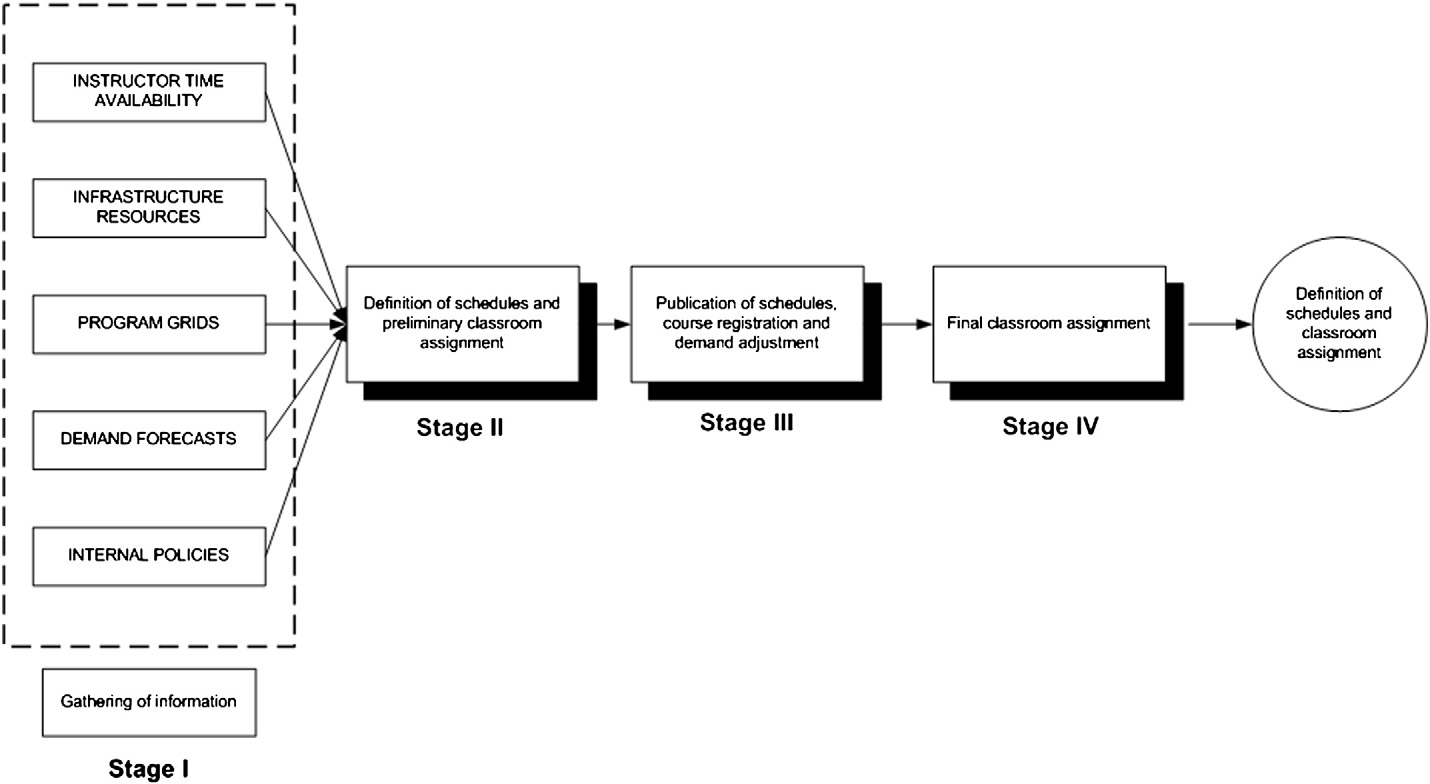
\includegraphics[width=\textwidth]{files/img/2.02!4-modelagem/Arquitetura-UDP}
  \legend{Fonte: \citeonline{miranda_udpskeduler_2012}}
\end{CenteredFigure}

Na \autoref{fig:geral}, estão dispostos 4 estágios principais. O primeiro dispõe da aquisição de informações, sendo elas a disponibilidade do profesor, os recuresos da infraestrutura, as grades dos cursos, as estimativas de demanda e as políticas internas. No segundo estágio são definidas grades horárias preliminares com atribuição preliminar das salas. No terceiro, os alunos se inscrevem e a demanda é ajustada, por fim, no quarto estágio, ocorre a alocação final das salas. Com sua conclusão, são definidos as grades horárias finais junto com as respectivas salas.

A sequência geral condiz com o processo de criação das grades horárias, porém é necessário adaptar a metodologia para o contexto da UENF, e também ao escopo do trabalho. Sendo assim, no primeiro estágio a coleta de informações sobre a disponibilidade dos professores e as matrizes curriculares dos cursos não será necessária. Os recursos de infraestrutura serão coletados dos histórico de alocação das turmas, a estimativa de demandas será obtida através da média histórica de alunos inscritos nas turmas e as políticas internas serão compreendidas através da revisão documental e entrevistas com os \textit{stakeholders}. O segundo tem caráter iterativo entre as coordenações e a diretoria do CCT. Os outros estágios não se distanciarão de forma significativa do que foi proposto.

\section{Iteração} % 4.2.

Para se alcançar uma alta satisfação por parte dos \textit{stakeholders}, vê-se necessária a constante interação com os mesmos. Para isto, será seguida a estrutura utilizada por \citeonline{andre_interaction_2018}.

\begin{MyCenteredFigure}
  \caption{Etapas do Design de Interação}
  \label{fig:IxD}
  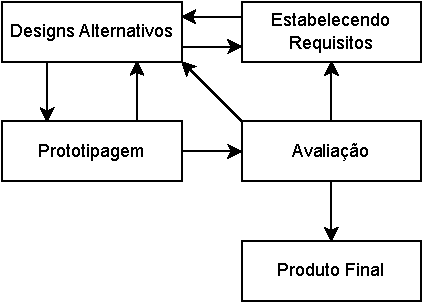
\includegraphics{files/img/2.02!4-modelagem/Arquitetura-IxD.drawio}
\end{MyCenteredFigure}

Seguindo o conceito do Design de Interação, a \autoref{fig:IxD} ilustra o ciclo de ações a serem tomadas durante o desenvolvimento do sistema, caso este venha a ser necessário. Nesse modelo de pesquisa, os \textit{stakeholders} serão consultados continuamente enquanto lhes for apresentados protótipos do sistema, para que assim informem quanto às suas percepções. Esta dinâmica tem como finalidade encontrar um design tal que seja adequado aos desejos e necessidades de seus usuários. Pois, considerando que para que o sistema seja efetivo, é necessário que ele seja aceito e utilizado pelos usuários finais.

\section{Funcionamento} % 4.3.

O sistema proposto funcionará de forma a auxiliar a coordenação do curso de Ciência da Computação da UENF criação de grades horárias para os semestres letivos. Para isso, o sistema deverá ser capaz de gerenciar as informações referentes às disciplinas, professores, salas e horários disponíveis.

Para tanto, mesmo que disponha de informações pré-cadastradas, o sistema deverá permitir a inserção de novas informações, como disciplinas, professores e salas, pois, apesar de não ser o foco principal do sistema, é recorrente que haja alterações nessas informações ao longo do tempo, e caso o sistema não as comporte, não poderá cumprir seu propósito.

Como forma de agregar as informações cadastradas, o usuário será capaz de criar turmas para as disciplinas, informando o professor responsável, a sala e o horário em que a turma ocorrerá. Além disso, o sistema deverá permitir a visualização das turmas já cadastradas, bem como a edição e exclusão das mesmas, caso necessário. Ao criar uma turma, o sistema viabiliza a definição de qual ano e semestre a turma pertence.

As turmas contarão também com a informação de demanda estimada, que será utilizada como comparativo para a alocação das salas, de forma a evitar que uma sala seja alocada para uma turma cuja demanda seja maior do que a capacidade da sala. Outra informação contida nas turmas será um código descritor da turma em questão. Esse código será utilizado para auxiliar na compreensão das turmas, visto que ao longo do processo de criação das grades horárias é recorrente a criação de turmas criadas com um propósito específico, como por exemplo contemplar apenas repetentes ou alunos de um determinado conjunto de cursos.

Como ponto chave do funcionamento do sistema, o mesmo deverá ser capaz de ilustrar conflitos que vierem a surgir durante a alocação dos recursos. Esses conflitos podem ser de diversas naturezas, como por exemplo, a alocação de uma turma em um horário em que o professor responsável não está disponível, ou a alocação de duas turmas em uma mesma sala e horário. A identificação desses conflitos é essencial para que a coordenação possa corrigí-los de forma prática e direta, assim evitando que ocorram problemas durante a execução das turmas no semestre letivo.

Por fim, o sistema viabiliza também um método de rápida criação de turmas para todas as disciplinas esperadas para determinado semestre letivo para o curso de Ciência da Computação. Esse método consiste em analisar as disciplinas esperadas para os estudantes de computação em determinado semestre letivo, e, através do cálculo das maiores recorrências de professor, sala e horário atribuídos às turmas dessa mesma disciplina em semestres anteriores, criar uma turma com essas informações. Esse método visa agilizar o processo de criação das turmas, visto que a coordenação não precisará criar cada turma manualmente, mas sim apenas revisar as informações geradas pelo sistema.

Dispondo de todas essas funcionalidades, o sistema deverá ser capaz de gerar uma grade horária final, que será utilizada como base para a criação da grade horária oficial do curso de Ciência da Computação da UENF.

\section{Modelo de Banco de Dados} \label{sec:ModelagemBD} % 4.4.

Considerando as informações necessárias para o presente trabalho, e também o preparo de campo para potenciais aplicações futuras, foi elaborado um diagrama conceitual de banco de dados, que pode ser visto na \autoref{fig:DiagramConceitual}.

\begin{MyCenteredFigure}
  \caption{Diagrama Conceitual do banco de dados}
  \label{fig:DiagramConceitual}
  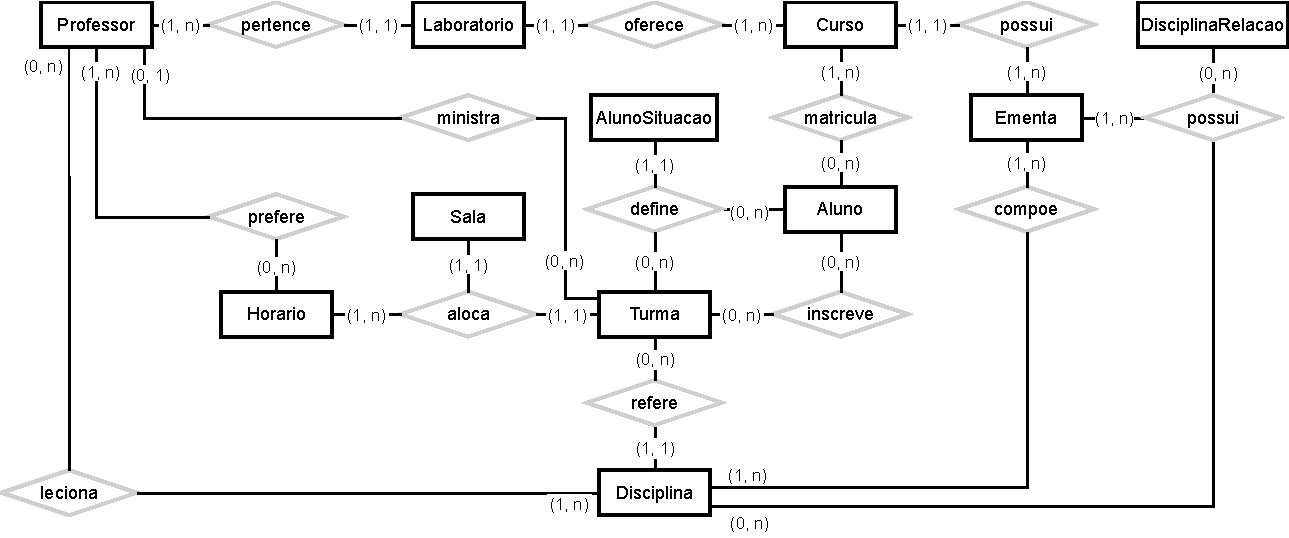
\includegraphics[width=\textwidth]{files/img/2.02!4-modelagem/Diagrama ER-Conc. Card.drawio}
\end{MyCenteredFigure}

O diagrama conceitual foi elaborado utilizando a ferramenta \LinkToURL{https://www.drawio.com}{draw.io} citada na metodologia e ilustra as relações entre diversas entidades presentes na realidade da UENF. O emaranhamento presente no diagrama ilustra a complexidade envolvida na criação de uma grade horária, onde diversas entidades se relacionam entre si.

Como principais apontamentos, podemos citar a parte principal do modelo que é a alocação de turmas. Ela, como já descrito, envolve a correlação entre alunos de diferentes cursos, professores, disciplinas, salas e horários. Além disso, também é possível notar a presença de entidades que não são diretamente relacionadas à alocação de turmas, mas que podem se mostrar úteis, como a relação entre professores e laboratórios, e a de disciplinas e ementas.

Embora o diagrama apresente uma visão mais completa de todas as interconexões possíveis, é importante ressaltar que o presente trabalho foca primordialmente na alocação das turmas para o curso de Ciência da Computação, e que a implementação do banco de dados será feita de forma a atender a essas necessidades, fazendo então uso de apenas uma parte do diagrama conceitual apresentado pela \autoref{fig:DiagramConceitual}.

\subsection{Diagrama de Entidade e relacionamento} % 4.4.1.

Neste modelo, mais enxuto, temos apenas as entidades principais, onde temos uma turma de determinada disciplina, ministrada por um professor e que ocorre em uma sala em um determinado horário.

Neste diagrama vemos as entidades principais, que são \textbf{Turmas}, \textbf{Disciplinas}, \textbf{Professores}, \textbf{Horários} e \textbf{Salas}. As propriedades escolhidas para cada entidade são compostas por uma mistura de critérios. Por exemplo, o nome do professor, o código da disciplina, e a junção de código e bloco auxiliam primordialmente na identificação real dos professores, disciplinas e salas. Já as informações ``período'', ``apelido'' e ``comment''...

E também é notável a presença da entidade \textbf{Alunos}, que se apresenta desacoplado das demais entidades. O motivo para isso é que, embora os alunos façam parte do processo de alocação de turmas, ao longo do desenvolvimento, o desenvolvimento de funcionalidades envolvendo os alunos...
